\section{Results}

Following the methodology described in the previous section, we estimate the total U.S. Resource to be 3700 $\pm$400 TWh/yr (Table~\ref{table:totals}). This is nearly double the total U.S. wave resource estimated in EPRI 2011. This result, however, is due to two mutually supportive changes to the methodology: 1) the extension of the assessment to the edge of the EEZ, and 2) the inclusion of the local resource in the total. The third fundamental change to the methodology -- utilizing a one-way dot-product -- actually reduces the resource estimates compared to EPRI 2011, but that change is overwhelmed by the increases due to the other changes.

In order to understand the source of these changes, we begin by comparing the EPRI 2011 results to the new remote results. Their are two primary differences in methodology between these two estimates: 1) the new remote results are based on a one-way vector line-integral, rather than the now debunked ``unit-circle method'', and 2) the new results use the edge of the EEZ as the integration contour, while the EPRI 2011 results utilized the 100-m isobath \note{something else in Gulf?}. \note{Do we also need to mention minor differences in method: different model and duration?} The first of these changes leads to a reduction in total resource, while the second changes the result in proportion to the change in the length of the contour.

Al

The EPRI 2011 assessment had three distinct differences from the current approach: 1) it computed only the remote resource, 2) it did so along the 100-m isobath, and 3) it utilized a 'unit-circle' line-integral method that was critiqued for `double-counting'. 
the revised methodology proposed herein, which is focused primarily on establishing a consistent and comprehensive methodology, rather than a fundamentally new understanding of wave physics. In other words, this work has not ``discovered new wave energy'', so much as modified the methodology to account for the wave energy potential over the entirety of the U.S.'s EEZ.

In particular, the addition of the local resource 

This increase is a result of changes to the methodology we've proposed. On one hand, 
but most of this increase is due to adding the local resource over the U.S. EEZ to the total, which was not included in the EPRI 2011 assessment. 


The EPRI 2011 resource assessment was different from this work in three important ways:
\begin{itemize}
\item It did not account for wave directionality.
\item It computed the wave resource along the 100m isobath, rather than the full EEZ.
\item It did not account for the local resource.
\end{itemize}
A comparison of the remote resource estimated here is a 

in the resource gains Roughly half of this is contained in the remote resource, and the other half is due to the local resource. 

Nearly two-thirds of this resource is in Alaska where a large resource area and energetic waves in the North Pacific combine to create a large total. The U.S. West Coast has a large remote resource where energetic waves from the North Pacific arrive from offshore.  The West Coast remote resource is, relatively, modest. The U.S. East Coast resource, on the other hand, is composed primarily of the local resource and has a relatively modest remote portion. This is because mid-latitude westerly winds tend to generate wave energy that propagates eastward, and relatively less wave energy from the open ocean propagates onshore from the open ocean (compared to the West Coast). This also indicates that much of the East Coast wave resource is located farther from shore, where there is sufficient fetch to have generated the wave energy that tends to be propagating eastward. \note{Is that last sentence accurate? Assuming yes, is a citation needed for that or is it `simple physics'-enough to simply be stated?}

Hawaii has a large resource due largely to waves that arrive from the North Pacific along the northern boundary of the EEZ surrounding the islands. The natural local resource is relatively small, due primarily to the fact that the sea-state in this region is -- in the long-average perspective presented here, and compared to regions such as the East Coast where wave growth dominates, or compared to the `potential' case -- roughly `steady-state' because the wind input and dissipation are relatively balanced. The Caribbean region (Gulf of Mexico, Puerto Rico, and U.S. Virgin Islands) on the other hand, has a modest wave resource composed predominantly of local wind input. \note{Is ``the Caribbean region'' a term, or is there something better I should use?} The remote resource of this region is also very small because the majority of the U.S. EEZ boundary throughout this region borders other EEZs (rather than being exposed to the open ocean), and the methodology described here only counts wave energy crossing into the EEZ from the open-ocean.

\begin{table}[ht]
  \centering
  \begin{tabular}{|c|c|c|c|c|c|}
    \hline
    %\multirow{2}{*}{Region}
    Region & {\it EPRI 2011}  & Remote & \multicolumn{2}{c|}{Local} & Total \\
    & {\it Remote} & & Natural & Potential & \\
    \hline
    Alaska & 1570 & 1040 & 990 & 1510 & 2030 - 2550 \\
    West Coast & 590 & 420 & 90 & 210 & 510 - 630 \\
    Hawaii & 130 & 370 & 10 & 100 & 380 - 470 \\
    East Coast & 240 & 110 & 180 & 230 & 290 - 340 \\
    Gulf of Mexico & 80 & 13 & 56 & 57 & 69-70 \\
    P.R. \& U.S.V.I. & 30 & 6 & 11 & 27 & 17 - 33 \\
    \hline \hline
U.S. TOTAL & 2640 & 1960 & 1340 & 2130 & 3300 - 4090 \\
\hline
  \end{tabular}
  \caption{Wave resource assessment results by region and totaled for the entire U.S. (all values in TWh/yr). The range in the total column indicates the sum of Remote+Local (lower value) and Remote+Potential (higher value). \note{Do we need to be more careful w/ significant digits here?}}
  \label{table:totals}
\end{table}

\note{Need to work on this...}
The large increase in resource in Hawaii is due in large part due to the exteneded area of integration. In the EPRI 2011 report the integration was performed at the 200 m isobath, which in the case of Hawaii is very close to shore due to the lack of continental shelf. In the present case, integration contour is extented to the EEZ which lies at 200 nmi in the Northern, Eastern, and Southern boundaries.

\begin{figure}[ht]
  \centering
  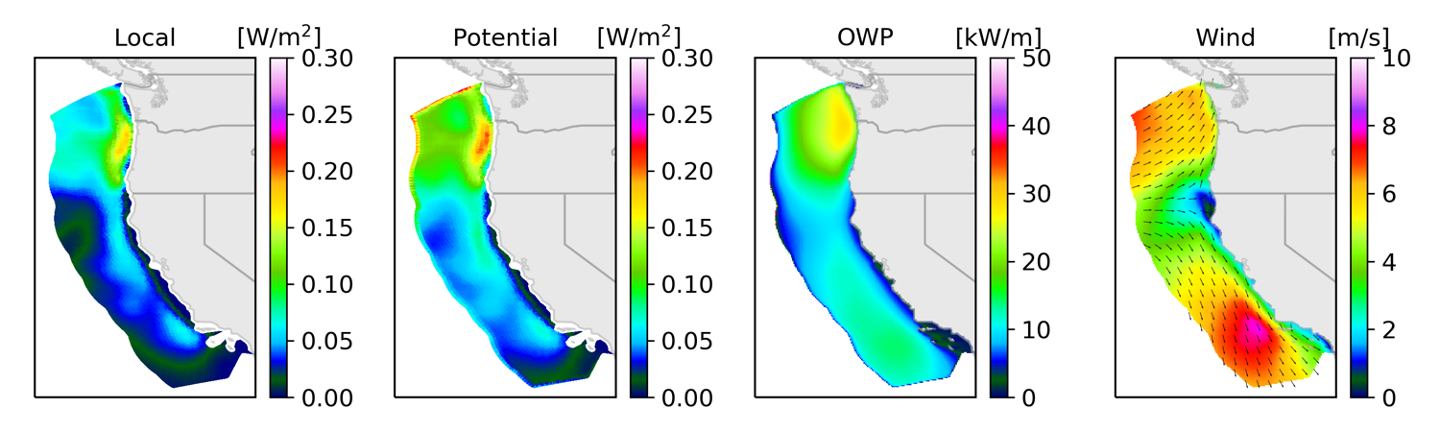
\includegraphics[width=\textwidth]{../fig/WC-Map01-November.png}
  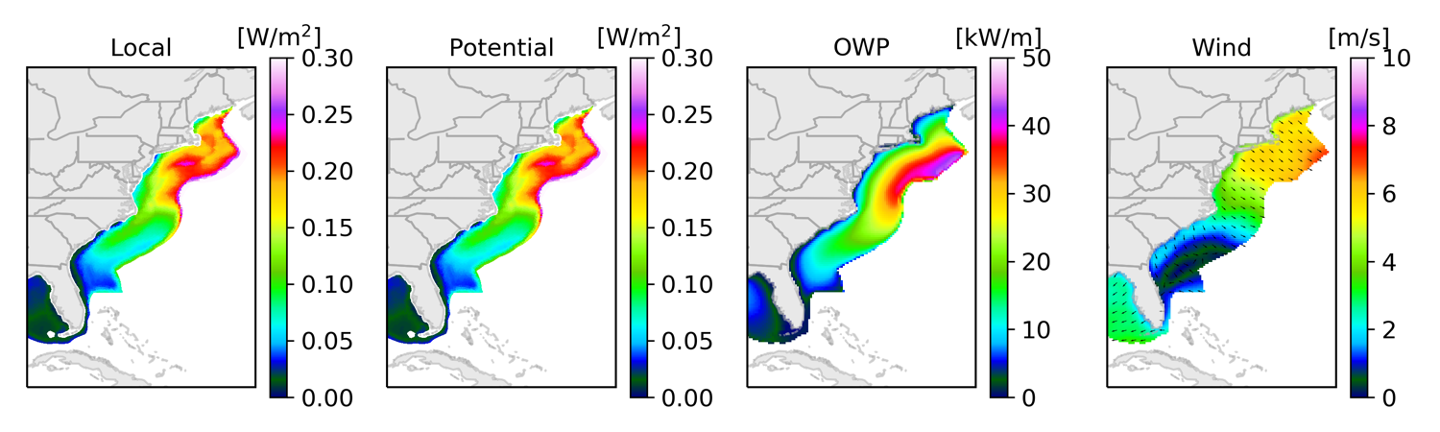
\includegraphics[width=\textwidth]{../fig/EC-Map01-November.png}
  \caption{Maps of wave resource for the West Coast (top), and East Coast (bottom). \note{GGM: Can we get these as total annual averages, or are those `boring'? Can we add mean wave-direction to the OWP plot?}}
  \label{fig:maps}
\end{figure}

\note{GGM: Regarding Figure \ref{fig:maps}: why are winds and 'potential resource' so different on WC? I would think they would be more spatially correlated? Specifically: why is wind high off of S. Cali, but potential/local resource is highest offshore of OR/WA? ... I think you've answered this question before, but I forget.}

\begin{table}[ht]
  \centering
  \begin{tabular}{|c|c|}
    \hline
    Region & Inner-Shelf Resource \\
    \hline
    West Coast & 410 \\
    Hawaii & 120 \\
    East Coast & 90 \\
    Gulf of Mexico & 20 \\
    Alaska & 1100 \\
    P.R. \& U.S.V.I. & 20 \\
    \hline \hline
    U.S. TOTAL & 1800 \\
    \hline
  \end{tabular}
  \caption{Inner-shelf resource. \note{Do we want/need to include this? It probably belongs in a different table? Or does it make sense on it's own like this?}}
  \label{tab:nearshore-total}
\end{table}

\subsection{Annual cycle of wave energy resource}

The annual cycle of the wave energy resource has a remarkably consistent pattern across all U.S. regions (Figure \ref{fig:annual-cycle}). Wave energy is a late-fall and winter dominated resource. The resource peaks in December or January across all regions, and is at a minimum in summer months. The inter-annual variability of the monthly-averaged West Coast resource is small during summer months when the resource is small (Figure \ref{fig:wc-variability}). During energetic winter months, the monthly-averaged resource can vary by more than 50\%, but in general the interannual variability is less than 30\% of the month's mean. This suggests that during energetic winter months wave energy projects should be expected to deliver at least their annual mean, with the potential of providing up to three-times that value. \note{Is that last sentence a stretch? Am I glossing over too many details about site-specific variability and device performance characteristics?} However, more detailed analysis is required to demonstrate these characteristics at individual sites and for individual technologies. Other regions have similar variability characteristics (not shown for simplicity).

\begin{figure}[ht]
  \centering
  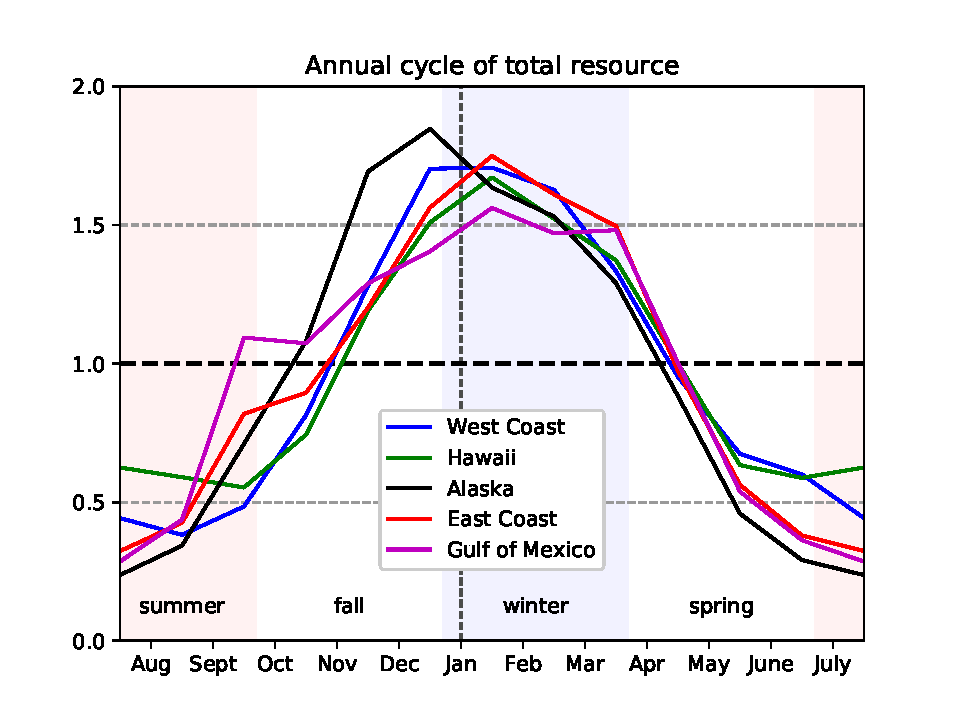
\includegraphics[width=\textwidth]{../fig/AnnualCycle01.pdf}
  \caption[Wave resource annual cycle.]{The annual cycle of the total wave energy resource for several regions, relative to the regional mean.}
  \label{fig:annual-cycle}
\end{figure}


\begin{figure}[ht]
  \centering
  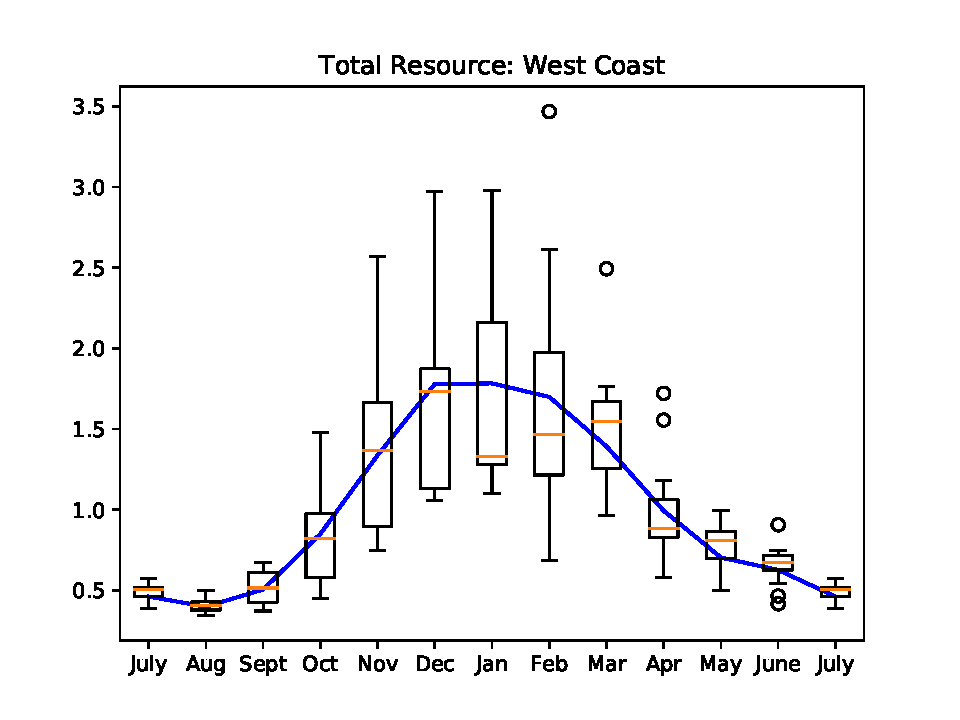
\includegraphics[width=\textwidth]{../fig/AnnualVar01.wc.pdf}
  \caption[West Coast resource variability.]{Annual and inter-annual variability of the West Coast resource. The thick solid line indicates the mean, and the orange lines and boxes indicate the median and quartiles, respectively. The whiskers extend to the last point within 1.5x of the inter-quartile range, and points beyond this are plotted as open-circles.}
  \label{fig:wc-variability}
\end{figure}

\begin{figure}[ht]
  \centering
  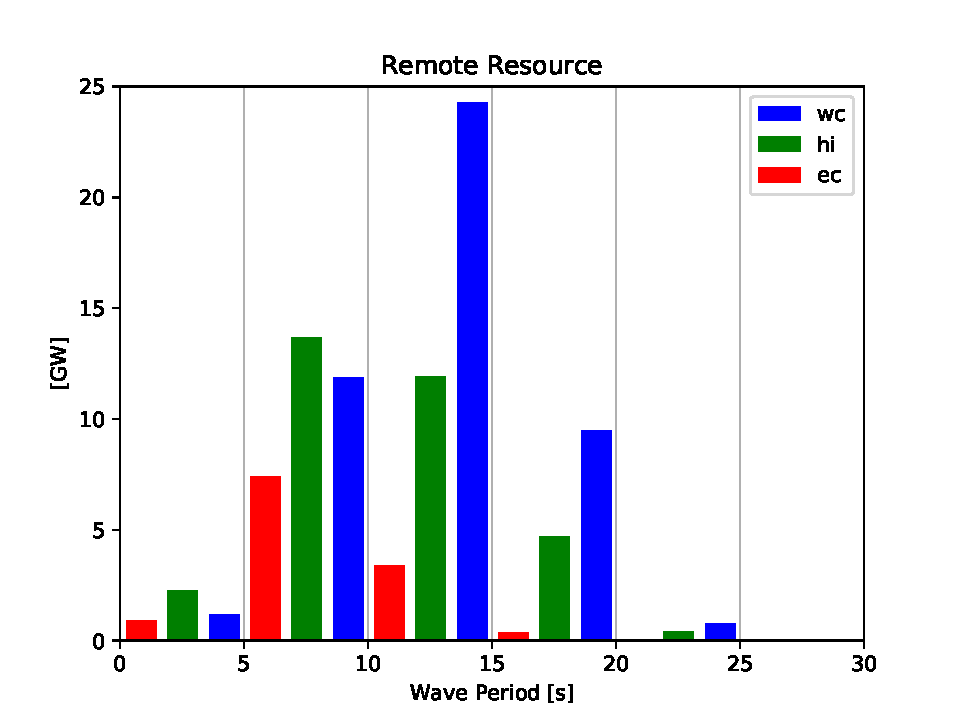
\includegraphics[width=\linewidth]{../fig/RemoteResource_Freq01.pdf}
  \caption{Remote resource contained in each wave period band (0-5 seconds, 5-10 seconds, etc.) for the west coast, Hawaii, and the east coast.}
  \label{fig:remote-freq}
\end{figure}

\begin{figure}[ht]
  \centering
  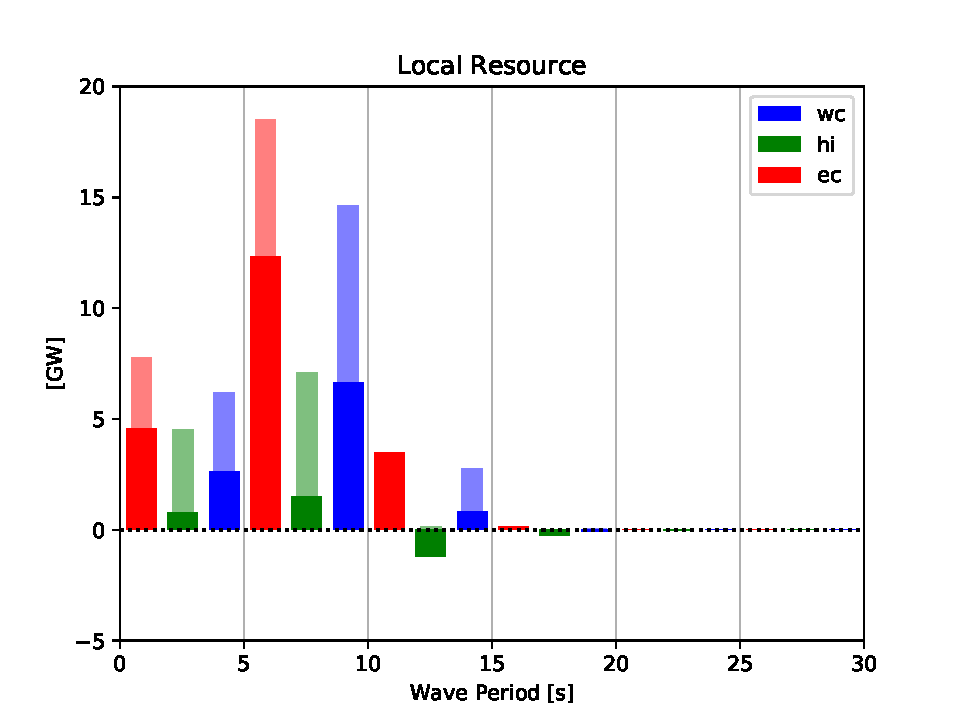
\includegraphics[width=\linewidth]{../fig/LocalResource_Freq01.pdf}
  \caption{Local (thick solid bars) and potential (narrow pale bars) resource contained in each wave period band (0-5 seconds, 5-10 seconds, etc.) for the west coast (wc), Hawaii (hi), and the east coast (ec).}
  \label{fig:remote-freq}
\end{figure}

\begin{itemize}
\item Maps of resource intensity (local + remote?)?
\item Frequency dependence of natural vs. potential. Natural has lower-frequency peak frequency \note{(right?)}, which means it is more likely to be useful energy. I.E. most of the `extra energy' in potential is rather high-frequency so maybe not so useful?
\item Plots of ‘remote’ resource vs. distance from shore (Figure 5). ... How does this compare with local resource vs. distance from shore?
\item Remote resource vs. depth. Local resource vs. depth.
\end{itemize}


%%% Local Variables:
%%% TeX-master: "wave_res"
%%% End:
